\documentclass[12pt]{article}
\usepackage[utf8]{inputenc}
\usepackage[T2A]{fontenc}
\usepackage[mongolian]{babel}
\usepackage{graphicx}
\title{Видео цомог}

\begin{document}
	\maketitle
	\begin{abstract}
		Хэрэглэгчийн шаардлага
	\end{abstract}

	\section{Функциональ шаардлага}
	\begin{itemize}
		\item Видео байршуулагчын ID 
		\item Видео байршуулагч видео байршуулах 
		\item Видео байршуулагч видео устгах
		\item Видео байршуулагч видео засах
		
		\item Гарчиг
		\item Хэмжээ
		\item Формат 
		\item Дэлгэцийн хэмжээ
		\item Насны ангилал
		\item Чанар (720,480,360)
		\item Лайк
		\item Үзсэн хүний тоо
		\item Дууны давтамж
	\end{itemize}
	
	\section{Функциональ бус шаардлага}	
	\begin{itemize}
		\item Хийсэн видеоны их бага  хэмжээ (100мб ч юмуу)
		\item Upload хийхэд ачааллах хурд

	\end{itemize}
	\section{Use case diagram}	
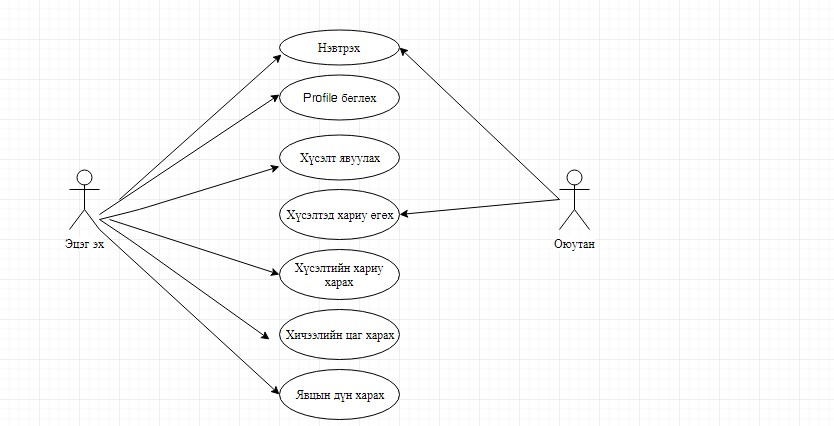
\includegraphics[scale=0.80]{images/usecase.jpg}

\end{document} 